\chapter{Method}
\label{chap:method}

\section{Design Goals}
\autoref{chap:related-work} reviewed existing approaches to reduce write amplification and their trade-offs.
We disclose the gaps in existing work that we aim to address in this thesis and identify the following design goals for our approach to reduce write amplification in B-Trees.

\subsection*{Reduce Write Amplification}
Write Amplification in B-Trees is primarily caused by the page-oriented design that requires rewriting entire pages to storage even if only a small portion changed.
This page-oriented design is crucial to utilize bandwidth of modern storage devices and to minimize buffer management overhead.
Merely reducing write amplification by reducing the amount of data written to storage is not the goal.
Instead, high write amplification suggests that we perform unnecessary writes to storage, which we would like to avoid.
We aim to mimimize the number of \ac{IO} operations induced by the B-Tree to perform a set of updates.
The overall goal is to create a B-Tree variant that is more write-efficient regardless of the access pattern.

\subsection*{Maintain Read Performance}
B-Trees are widely used in general-purpose database systems due to their excellent read performance for point lookups and range scans.
As we showed in \autoref{chap:related-work}, many write-optimized data structures sacrifice read performance.
For example the \ac{LSMT} incurs high read amplification to achieve high write-efficiency. 
The Bw-Tree introduces a delta chain to each node that needs to be traversed on every node read.
The BB$\epsilon$-Tree introduces an extra binary search for every node on the search path.
In contrast, we aim to keep the overhead of our optimizations minimal and preserve read performance of B-Trees.

\subsection*{Maintain Concurrency}
% Observation: The data structure itself should remain free of buffering logic to not compromise concurrency.
B-Trees are designed for high concurrency, allowing multiple threads to perform operations simultaneously.
Many write-optimized data structures compromise concurrency to achieve high write-efficiency.
For example, the B$\epsilon$-Tree introduces longer locking periods of the most frequently accessed nodes, reducing throughput in the tree.
In contrast, we aim to keep our optimizations outside of the data structure itself to not compromise concurrency of B-Trees.

\subsection*{Maintain Simplicity}
B-Trees are widely used in practice due to their simplicity.
Some write-optimized data structures, like the B-$\epsilon$-Tree, introduce significant complexity to the data structure itself.
In contrast, we aim to keep our optimizations lightweight, allowing for easy integration into existing systems.
The changes we introduce to the B-Tree itself should be minimal.
We aim to keep a low coupling between the data structure and the storage manager, allowing for optimizations in both layers independently.
Neither do we require special hardware features, making our approach broadly applicable across different storage media and hardware configurations.

% Idea: Introduce a layer between the data structure and the storage manager that buffers writes and applies them in batches.
% Minimal changes to the data structure itself. 
% Maintain Low Coupling between the data structure and the storage manager. Allows for optimizations in both layers independently like pointer swizzling.
% No invasive overhead.
% Not require special hardware features. Applicable to all storage media.


\section{High-Level Description of the Data Structure}

\begin{figure}[htpb]
  \centering
  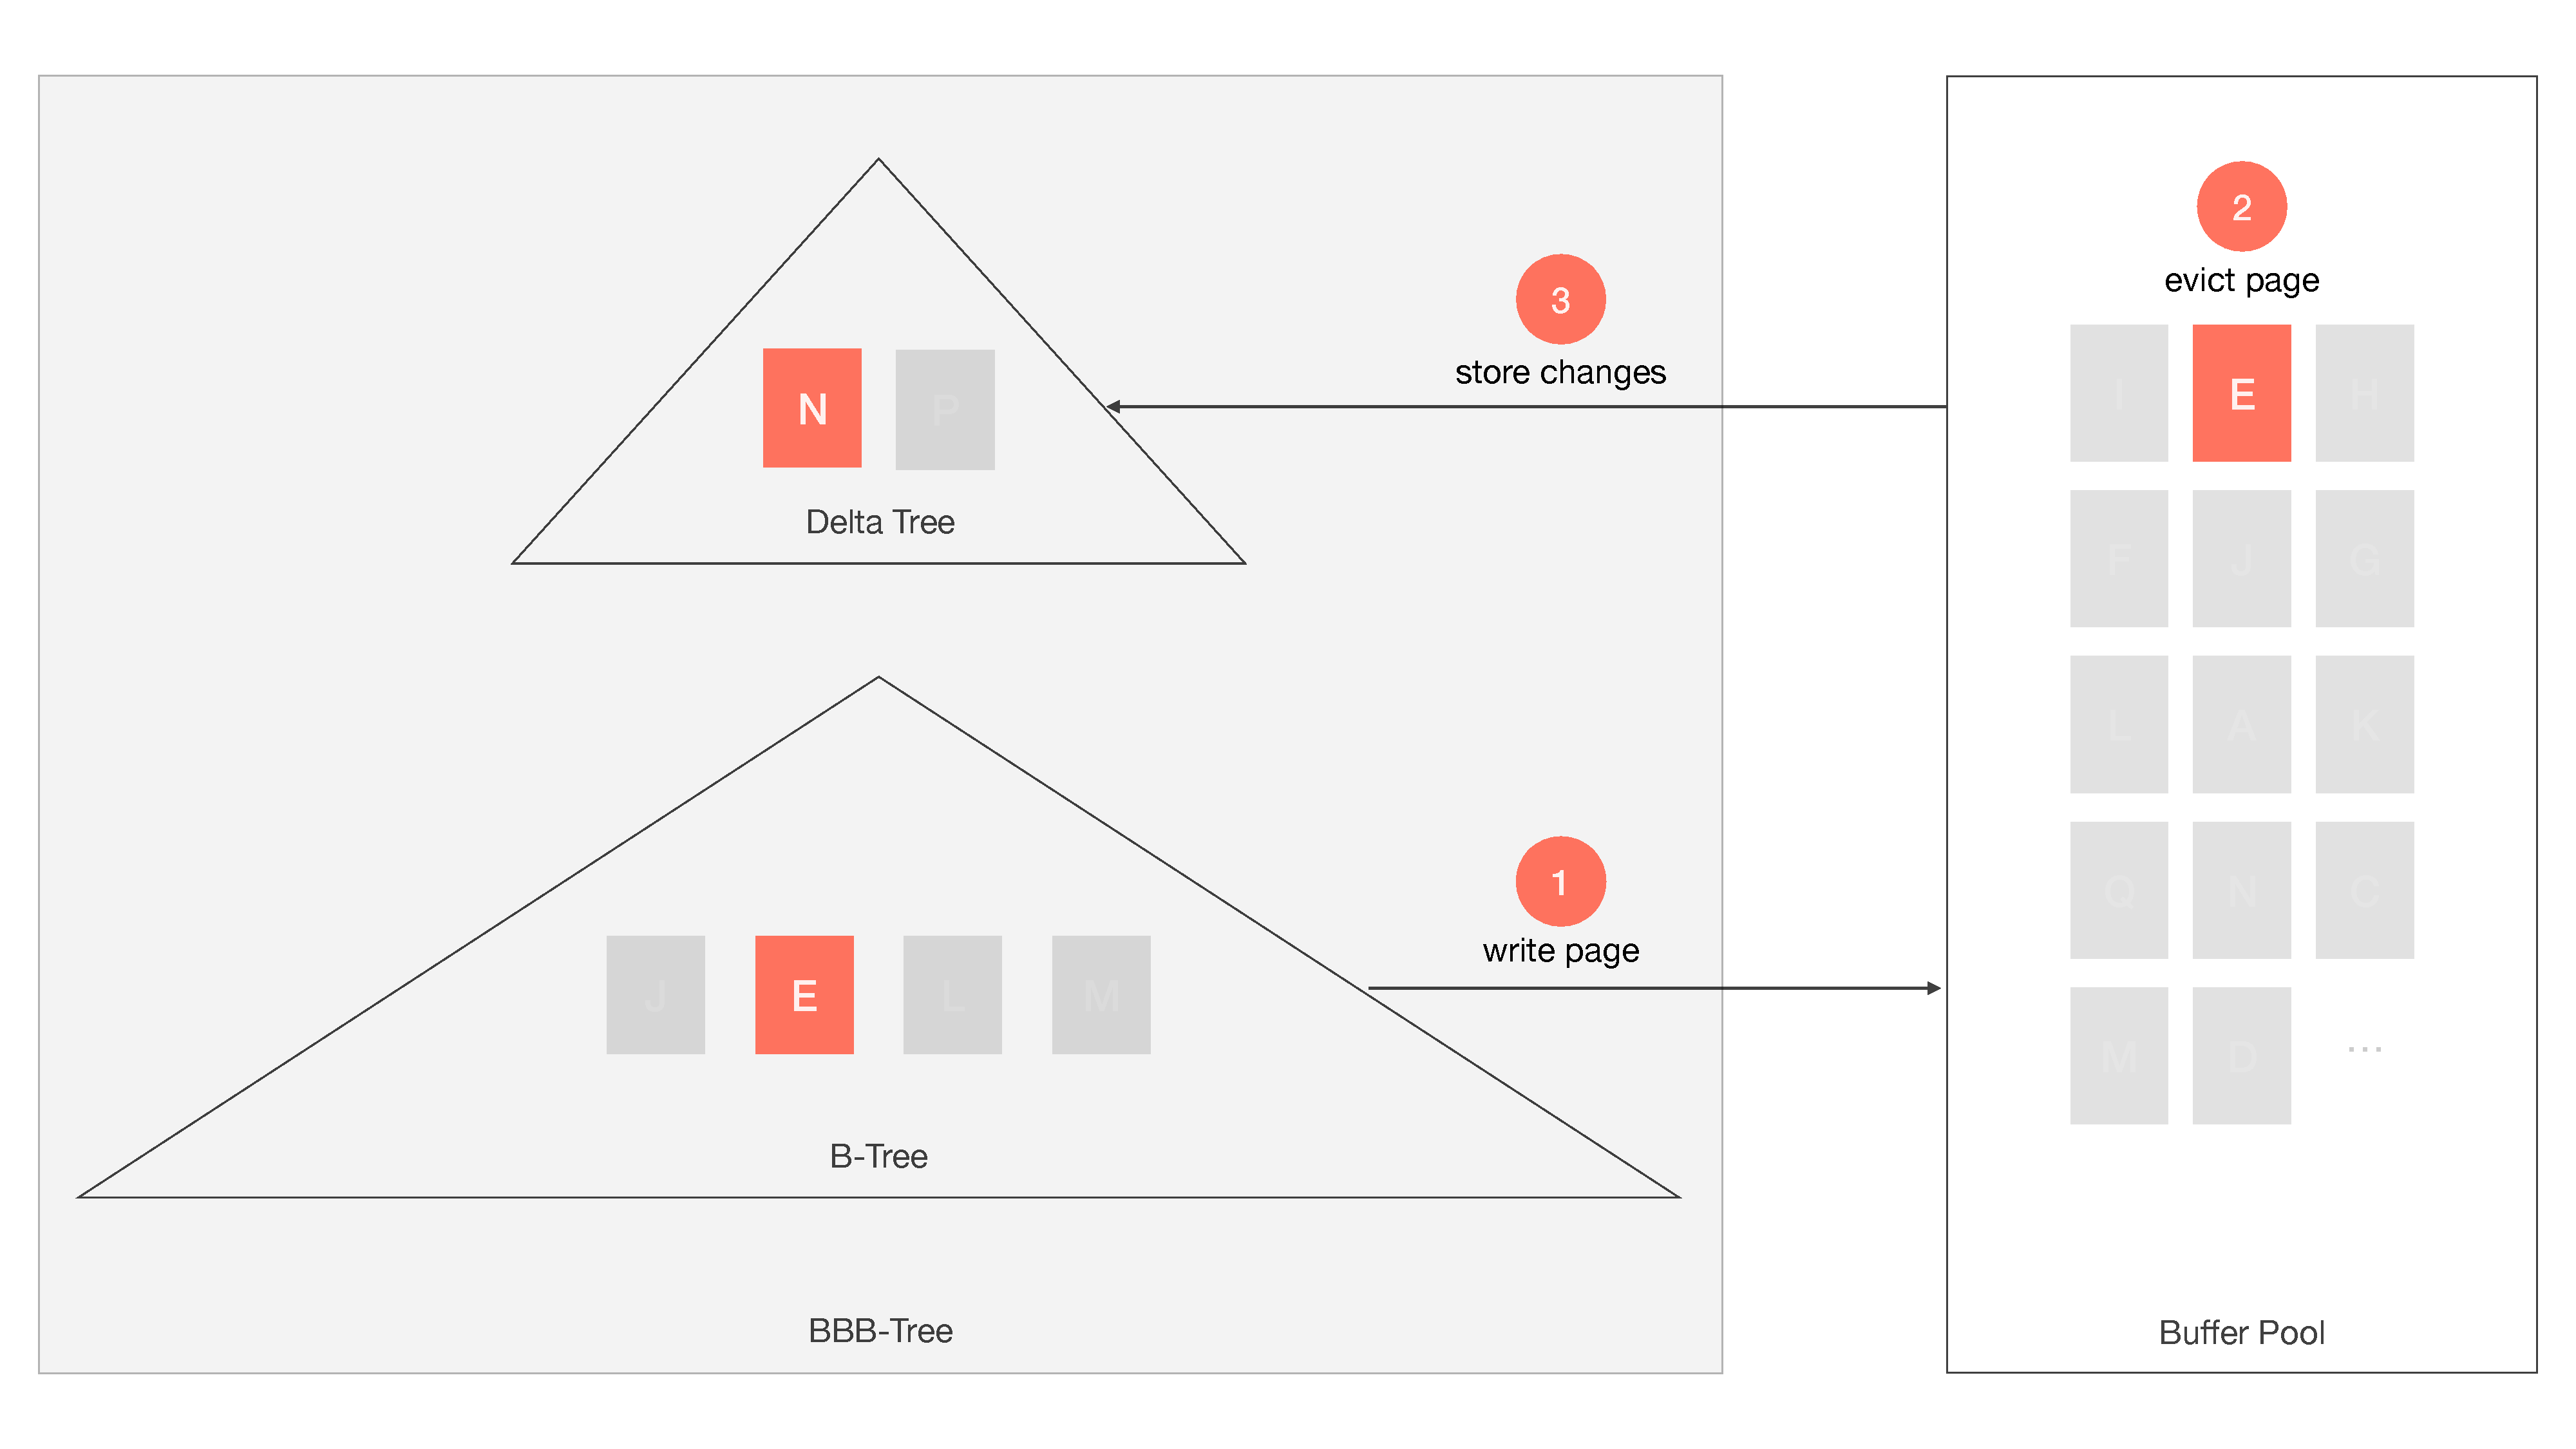
\includegraphics[width=0.99\textwidth]{figures/delta_tree.pdf}
  \caption{High-level architecture of the data structure. We add a Delta-Tree to a B-Tree. When evicting a dirty page from the B-Tree, we can buffer the changes of the B-Tree pages instead of writing them to storage. When loading a page from storage, we apply all buffered changes to it before returning it to the B-Tree.}
  \label{fig:delta-tree}
\end{figure}

We avoid writing a page to storage if changes are small.
To achieve this, we introduce a Delta Tree that acts as a hesitation layer, as illustrated in \autoref{fig:delta-tree}.
When evicting a dirty page, we can buffer the changes of the B-Tree pages instead of writing them to storage immediately.
We can just discard the page, saving us the write to storage.
When loading a page from storage, we apply all buffered changes to it before returning it to the B-Tree.
Only when enough changes accumulate, we write the full page to storage.

\inlinesection{Reduce Write Amplification.}
Write amplification in a B-Tree happens at the point of evicting a page to storage.
The buffer manager is only aware that a page is dirty and needs to be written to storage.
It does not know which parts of the page changed.
Therefore, we keep track of the modifications made to each page in the B-Tree.
Our component interacts with the buffer manager to intercept the eviction of dirty pages.
When evicting a dirty page, we can buffer the changes in the Delta Tree instead of writing them to storage immediately.
This way, we can defer small random writes until we have enough changes to justify a full rewrite to storage.
In the Delta Tree we can batch changes to the same page.

\inlinesection{Maintain Read Performance.}
To nodes in memory, this method is transparent.
When searching pages in memory, we do not incur overhead.

The only time we incur overhead is when loading a page from storage or unloading it to storage.
We argue that this overhead is acceptable, as we are already loading a page from storage.
The overhead of applying the buffered changes is small compared to the \ac{IO} operation.

However, the buffering layer itselt is a disk-based data structure, which migh require \ac{IO} operations to look up buffered changes.
We will be analyzing the overhead in \autoref{chap:evaluation}.    % TODO: Make sure that we do.
% i.e. there is an incentive to keep the delta tree small.
% TODO: Maybe we have more read amplifciation though because we also have IO to load the delta tree to apply changes.

\inlinesection{Maintain Concurrency.}
The Delta Tree is separate from the B-Tree.
Therefore, we do not compromise concurrency of the B-Tree itself, since we do not introduce further locking in the B-Tree itself.
The Delta Tree can be implemented as a B-Tree variant itself, allowing for high concurrency.

\inlinesection{Maintain Simplicity.}
The modifications we introduce to the B-Tree itself are minimal.
Within the B-Tree, we only need to track the modifications made to the nodes.
Essentially, we mark entries as dirty. 

The Delta Tree is a separate component that interacts with the buffer manager.
We do not dictate how the buffer manager is implemented or how it manages pages.
As a result, we maintain a low coupling between the data structure and the storage manager, allowing for optimizations in both layers independently.
For example, pointer swizzling is an optimization that could be applied with our method.

The Delta Tree itself is a B-Tree variant, which we already have present in our system.
Therefore, we can reuse existing code and concepts, reducing implementation complexity.
Neither do we assume any special hardware features, making our approach broadly applicable across different storage media.

% Learned from related work that we want to turn small writes into large sequential writes by batching them.
% Obervation: Write amplification in B-Trees is caused at the point of eviction. This is the point in time to buffer to defer a write.
% Uptain the happy path. We don't want any overhead for reads like a delta chain. At least not everytime we read from memory.

% Write out record-level updates on the page to another tree.
% A hesitation layer between B-Tree and buffer manager.
% A buffer that can defer the write of a B-Tree node. 
% When evicting a dirty page, we buffer the changes in memory instead of writing them to storage immediately.
% We can just discard the page, saving us the write to storage.
% To nodes in memory this is completely transparent. 
% Only when enough changes accumulate, we write the full page to storage. 
% When loading a page from storage, we apply all buffered changes to it before returning it to the B-Tree.
% This way, we can turn many small random writes into few large sequential writes.
% We use a B-Tree to buffer deltas. 

% Figure: Diagram of the architecture with the new layer.
\section{Data Structure Modifications}
% Figure: B-Tree and BBB-Tree (B-Tree plus its Delta Tree, called by the Buffer Manager)
\subsection*{Buffer Manager}
The buffer manager is the component that decides when a page is evicted from memory and when a page is loaded into memory.
At the same time, the buffer manager should not be aware of any semantics of its pages.
More specifically, it does not know if it is evicting or loading pages of a B-Tree or any other data structure.
However, we require specific logic to be executed when evicting or loading pages of a B-Tree.
We need a way to inject this logic into the buffer manager without leaking B-Tree specific logic into the buffer manager itself.
Therefore, users can register function pointers that are invoked at eviction time and loading time.
That way, the buffer manager remains agnostic of the semantics of its pages.

\subsection*{B-Tree}
\begin{enumerate}
  \item \textbf{Tracking Write Amplification:}
We need to be aware of the degree of write amplification per node. 
Whenever we modify a node, for example through an insertion or a node split, we keep track of the amount of bytes that were changed.
Then, in relation to the page size, we can determine the write amplification of the node.
Based on that parameter, we can decide if a write operation to external storage is justified, or if we want to defer it.
  \item \textbf{Tracking Deltas:} 
We need to determine the changes that occurred on a node since the last time it has been loaded from external storage.
To that end, each entry on a node has an additional "state" field that indicates if the entry was inserted, updated, or deleted since the last time the node was loaded from external storage.
That way, we can buffer the "delta" image of a node at eviction-time and apply it again at loading time to ensure that we can reconstruct the logical state of a node when it is accessed again at a later point in time.
\item \textbf{Injecting Callbacks:}
As described above, we need to execute specific logic at eviction time and loading time of a B-Tree page.
However, the B-tree has no control over the point in time a page is evicted or loaded.
Therefore, we inject callbacks into the buffer frames that are later invoked by the buffer manager.
Whenever we request a B-Tree page from the buffer manager, we register function pointers for the Delta Tree.
At eviction- and loading-time, these function pointers are called by the buffer manager to execute the necessary logic.
\end{enumerate}

Alternatively, we could have immediately inserted changes into the Delta Tree whenever a change occured on a B-Tree node.
This way, we would not need to track changes on the B-Tree nodes themselves.
However, this would introduce significant overhead on every write operation to the B-Tree.
Should a node be changed multiple times while it is in memory, we would need to update the Delta Tree multiple times as well.
In that case, we have many updates to a B-Tree node and therefore want to perform the write to storage anyway.
We would have introduced the most overhead for situations without any benefit.
Therefore, we only interact with the Delta Tree at eviction- and loading-time of a B-Tree page instead.
Only if we decide to buffer changes, we insert them into the Delta Tree.
This way, we keep the overhead for B-Tree operations minimal.

\subsection*{Delta Tree}
The Delta Tree is the component that buffers changes of B-Tree nodes.
The Delta Tree itself is a B-Tree with \ac{PID}s as keys and lists of changes as values.
The buffer manager calls back the Delta Tree everytime a dirty B-Tree page is evicted from memory or loaded into memory.

\begin{enumerate}
  \item \textbf{Eviction Time:}
The Delta Tree can decide if a B-Tree page should be written to storage or not based on the write amplification of the page.
Should it decide to not write the page to storage, it buffers its changes.
It does so, by scanning the node for entries that were marked as dirty and inserting them into its own B-Tree.
The buffer manager is informed that the page does not need to be written to storage anymore and can simply be discarded.

Should it decide to continue writing the page to storage, it simply returns and the buffer manager writes the page to storage as usual.
In this case, we clean the state of the B-Tree page and remove any buffered changes from the Delta Tree, as it is now in sync with storage.

  \item \textbf{Loading Time:}
When loading a B-Tree page from storage, the Delta Tree looks up if there are any buffered changes for that page.
If so, it applies the changes to the page before returning it to the B-Tree.
Together with the state of the page on storage, we can reconstruct the state of the page in memory.

When changes were applied, we keep them in the Delta Tree, as they might be useful for future evictions.
This way, we perform less updates to the Delta Tree and can keep the state of the B-Tree page clean.
Should there be no further changes to that page, the next eviction can simply discard the page without any writes.
\end{enumerate}

The Delta Tree itself contains pages that are managed by the buffer manager.
Its pages can be evicted to storage as well.
Therefore, we want to keep the Delta Tree small to batch changes more effectively.

\section{Implications on Write Amplification}
We can illustrate the effect of our approach on write amplification with a simple example.
\autoref{fig:delta-tree-example} shows a B-Tree with updates across three nodes with \ac{PID}s {1, 2, 4}.
In a traditional B-Tree, we would need to write all three pages to storage.
Assuming a page size of 4 KB and each update being 64 B, the write amplification is $(4096 B / 64 B) * 3 = 192$.

With our approach, we can buffer the changes of the three pages in the Delta Tree.
In this example, the Delta Tree only needs to write one page to storage, containing the three updates.
Assuming a page size of 4 KB again and approximating the delta entries to be 64 B each, the write amplification is now $4096 B / (3 * 64 B) = 21.33$.
In this simple example, we have reduced the write amplification by a factor of >9.

This demonstrates the goal of our approach: batching small writes on many distinct pages into larger writes on fewer pages.
This way, we can reduce the number of pages written to storage for a given set of updates, thereby reducing write amplification.

\begin{figure}[htpb]
  \centering
  \begin{subfigure}[t]{0.95\textwidth}
    \centering
    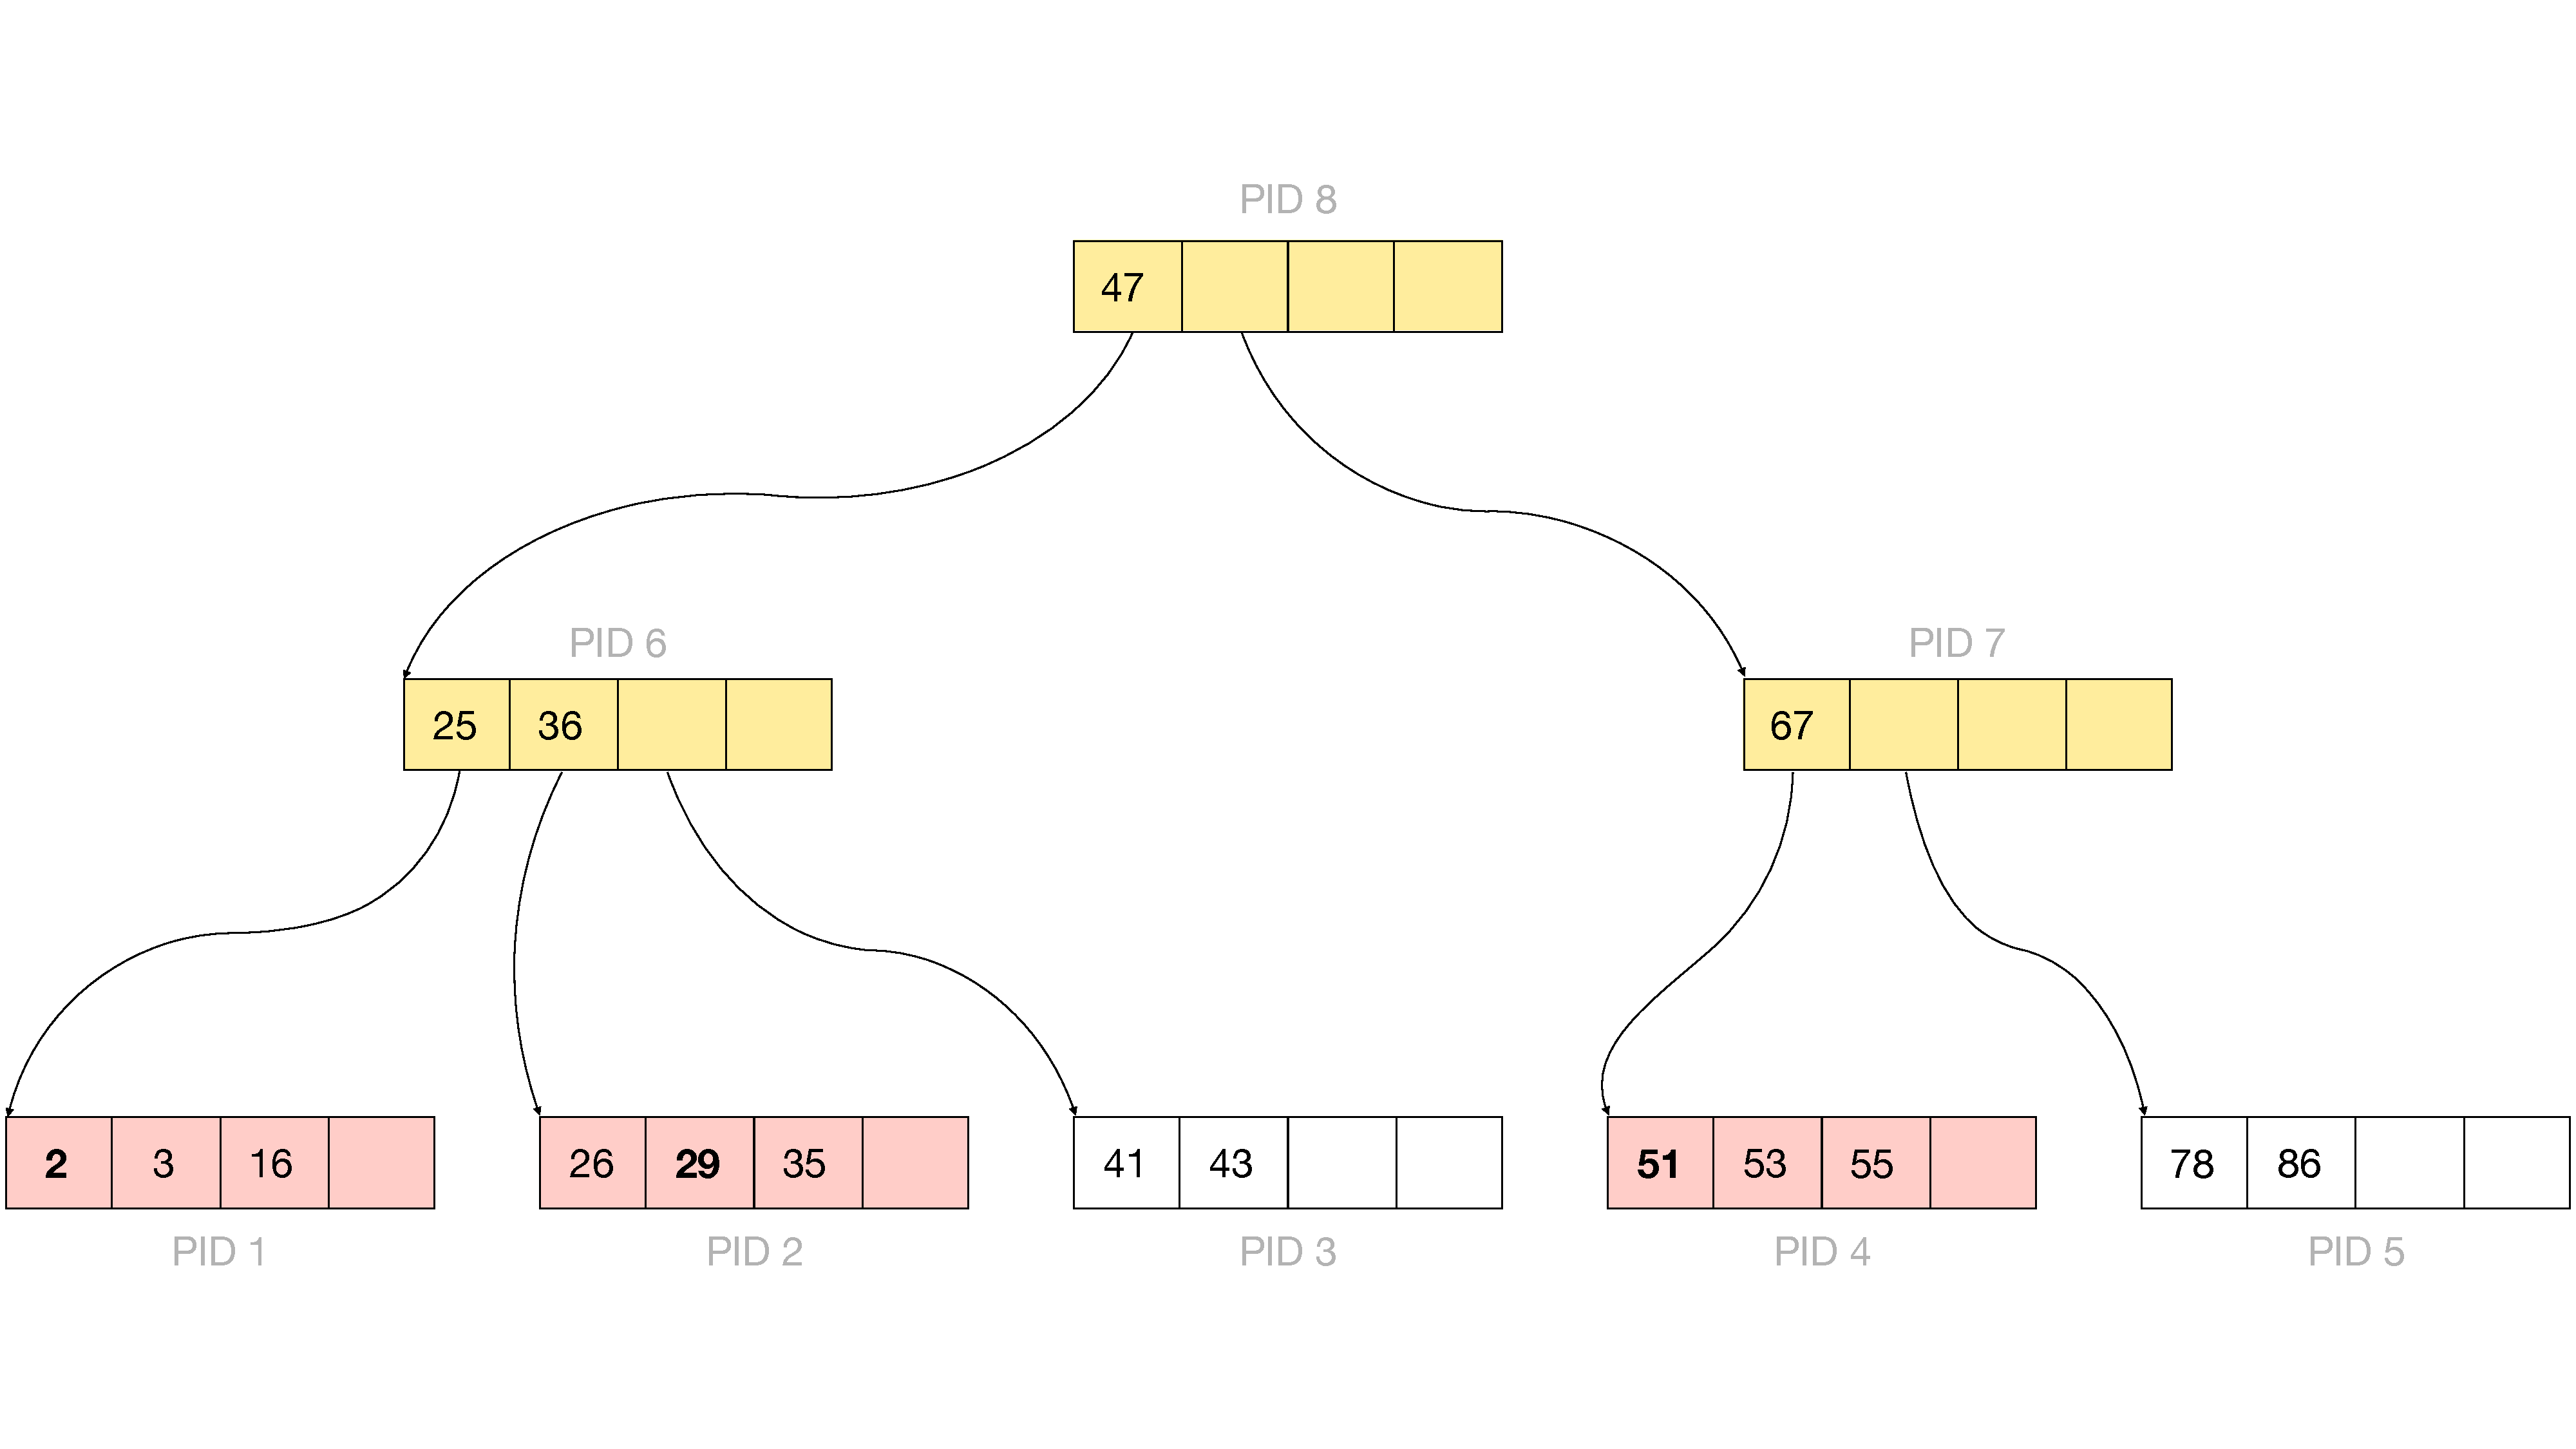
\includegraphics[width=\textwidth]{figures/b_tree_with_pid.pdf}
    \caption{A B-Tree with updates to nodes with \ac{PID} {1, 2, 4}.}
  \end{subfigure}
  \hfill
  \begin{subfigure}[t]{0.95\textwidth}
    \centering
    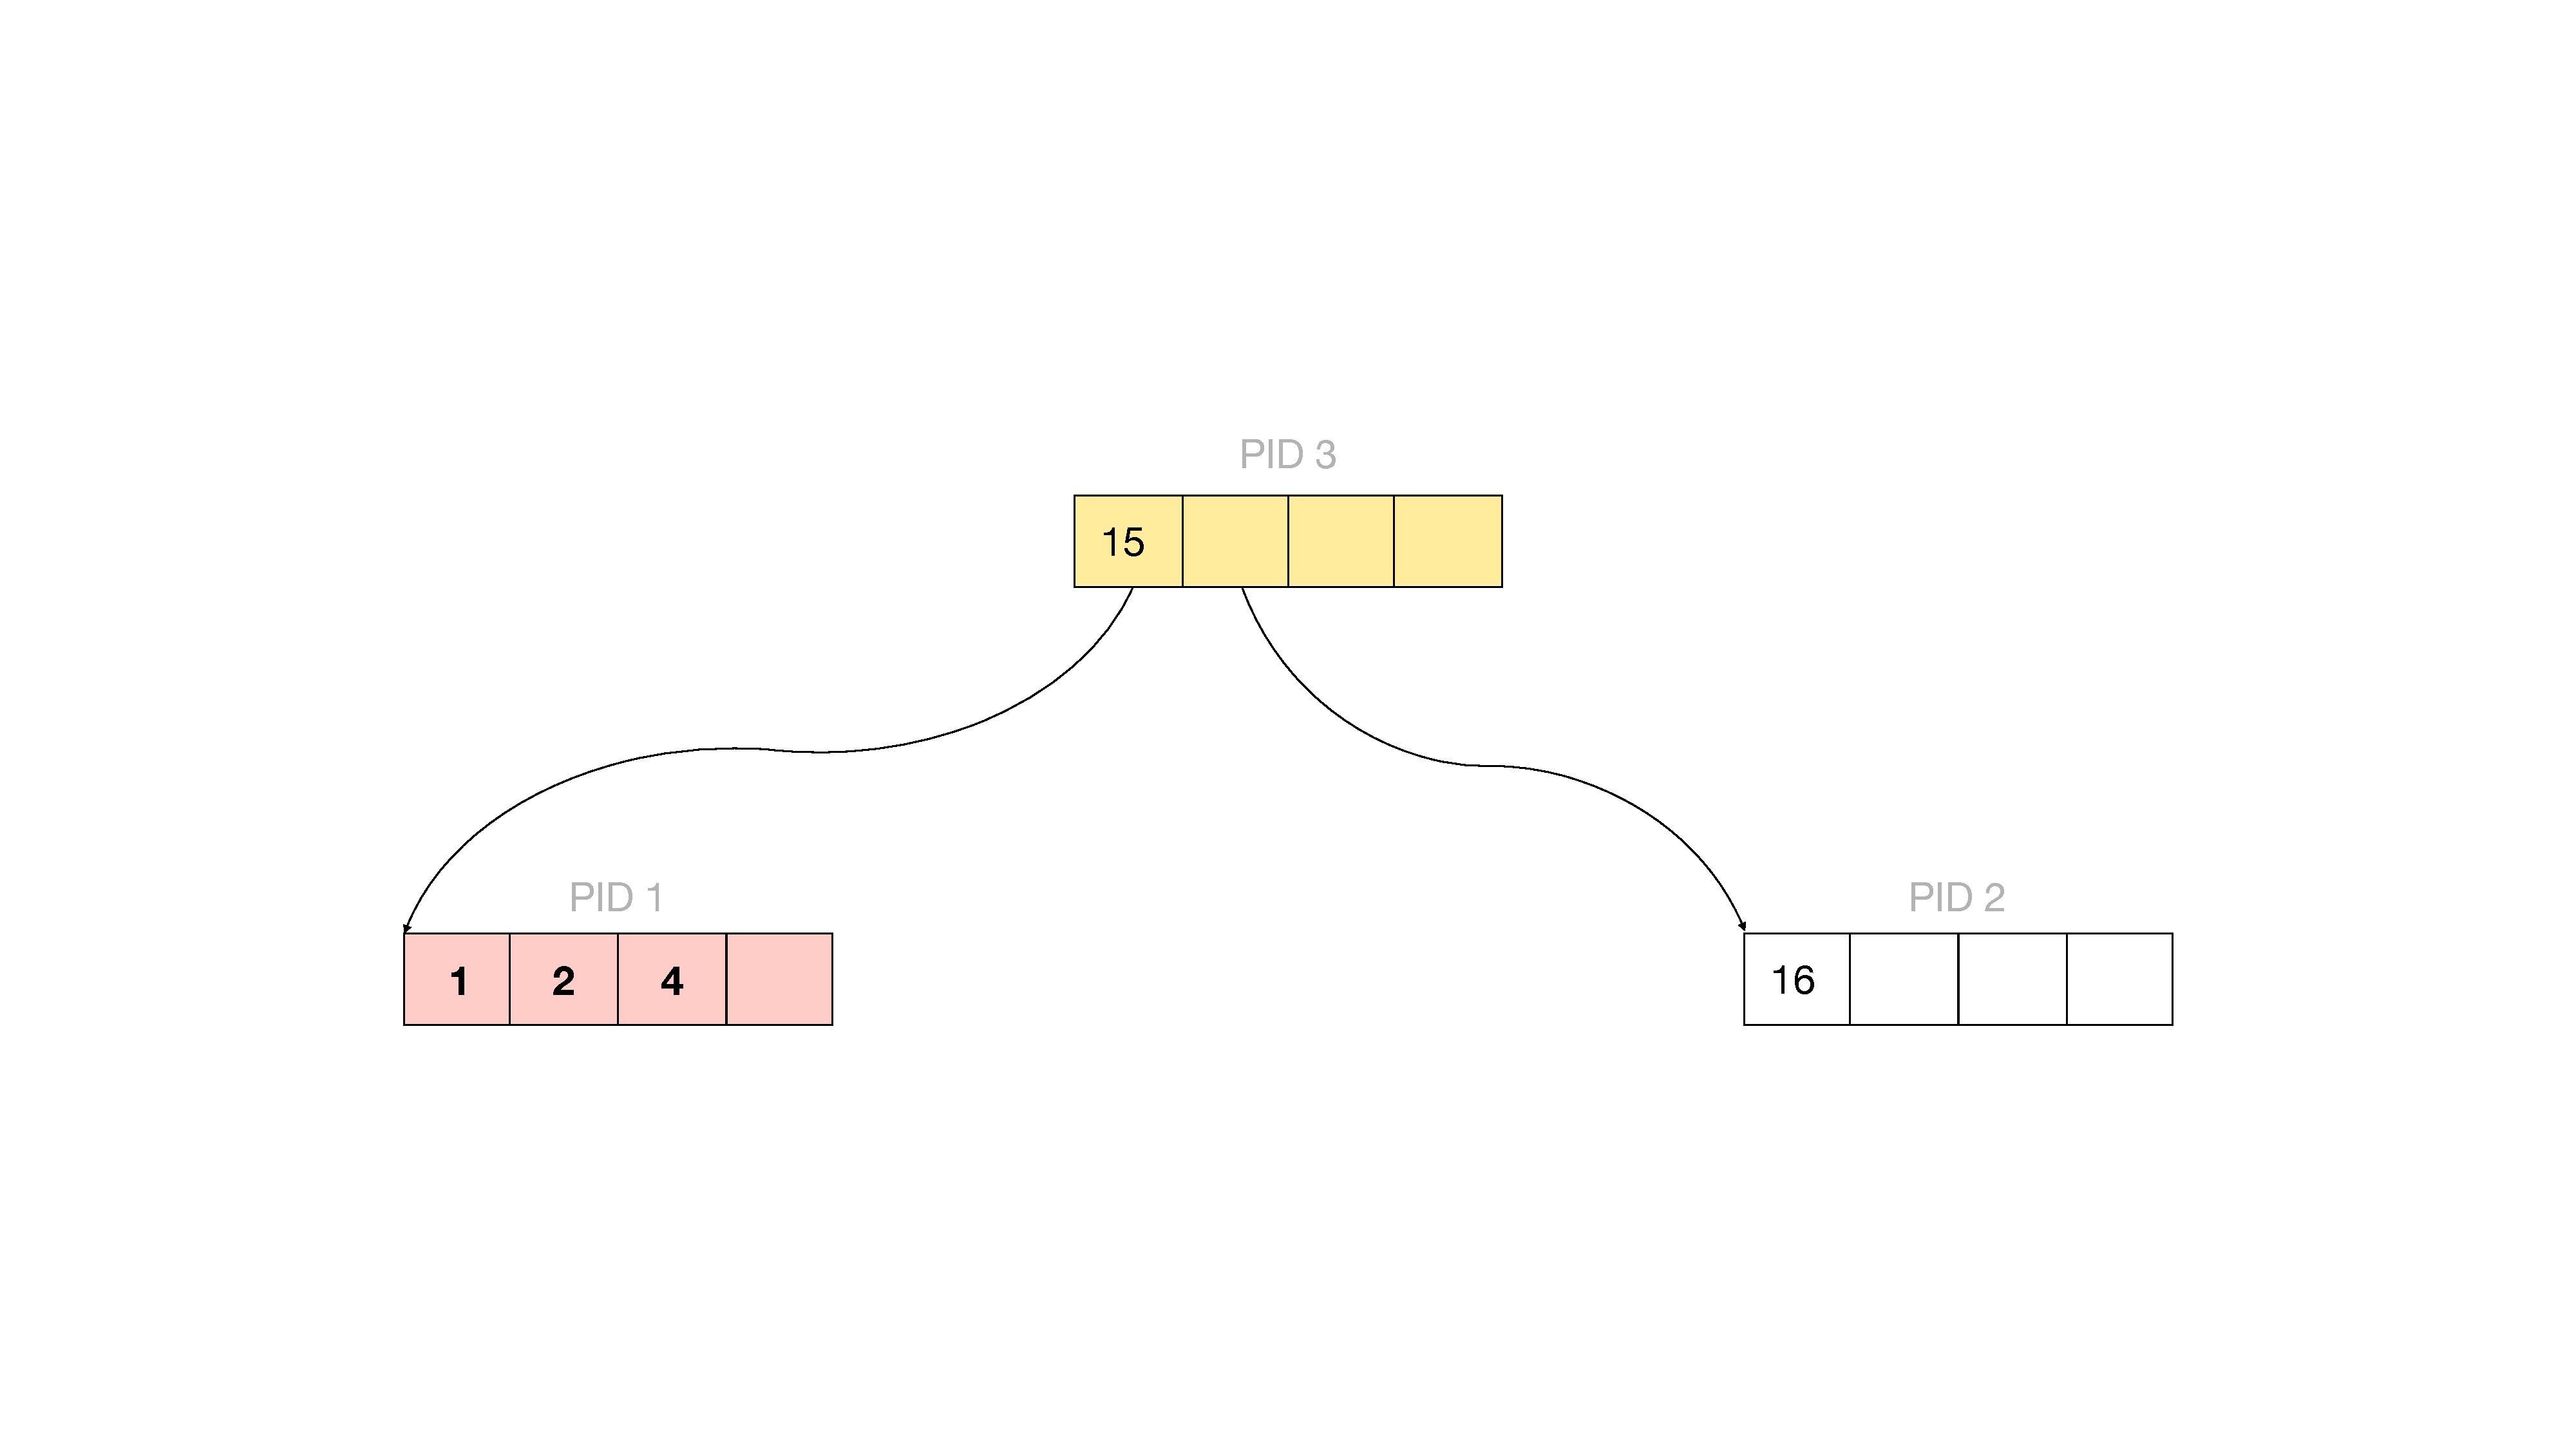
\includegraphics[width=\textwidth]{figures/delta_tree_update.pdf}
    \caption{The corresponding Delta Tree. Buffered the changes of B-Tree nodes by their \ac{PID}s {1, 2, 4}.}
  \end{subfigure}
  \caption{Example of a B-Tree and its corresponding Delta Tree. The B-Tree has three updated nodes marked in red. In this example, we require only one page write for the Delta Tree instead of three writes for the B-Tree.}
  \label{fig:delta-tree-example}
\end{figure}
